
\dataset{} facilities training agents for navigation, question asking, and question answering.
In this paper, we focus on navigation.
The ability to navigate successfully given dialog history is key to any future work in the Vision-and-Dialog Navigation paradigm.
Every dialog is a sequence of \nav{} question and \ora{} answer exchanges, with \nav{} steps following each exchange.
We use this structure to divide dialogs into \taskfull{} (\task{}) instances.

In particular, \dataset{} instances are each comprised of a repeating sequence ${<N_0, Q_1, A_1, N_1, \dots, Q_k, A_k, N_k>}$ of navigation actions, $N$, questions asked by the \nav{}, $Q$, and answers from the \ora{}, $A$.
Because sending a question or answer ends the worker's turn, every question $Q_i$ and answer $A_i$ is a single string of tokens.
For each dialog with prompt $(S, t_o, p_0, G_j)$, an \task{} instance is created for each of $0\leq i\leq k$.
The input is $t_o$ and a (possibly empty) history of questions and answers $(Q_{1:i}, A_{1:i})$.
The task is to predict navigation actions that bring the agent closer to the goal location $G_j$, starting from the terminal node of $N_{i-1}$ (or $p_0$, for $N_0$).
We extract 7415 \task{} instances from the 2050 navigation dialogs in \dataset{}.

\begin{figure}[ht]
\centering
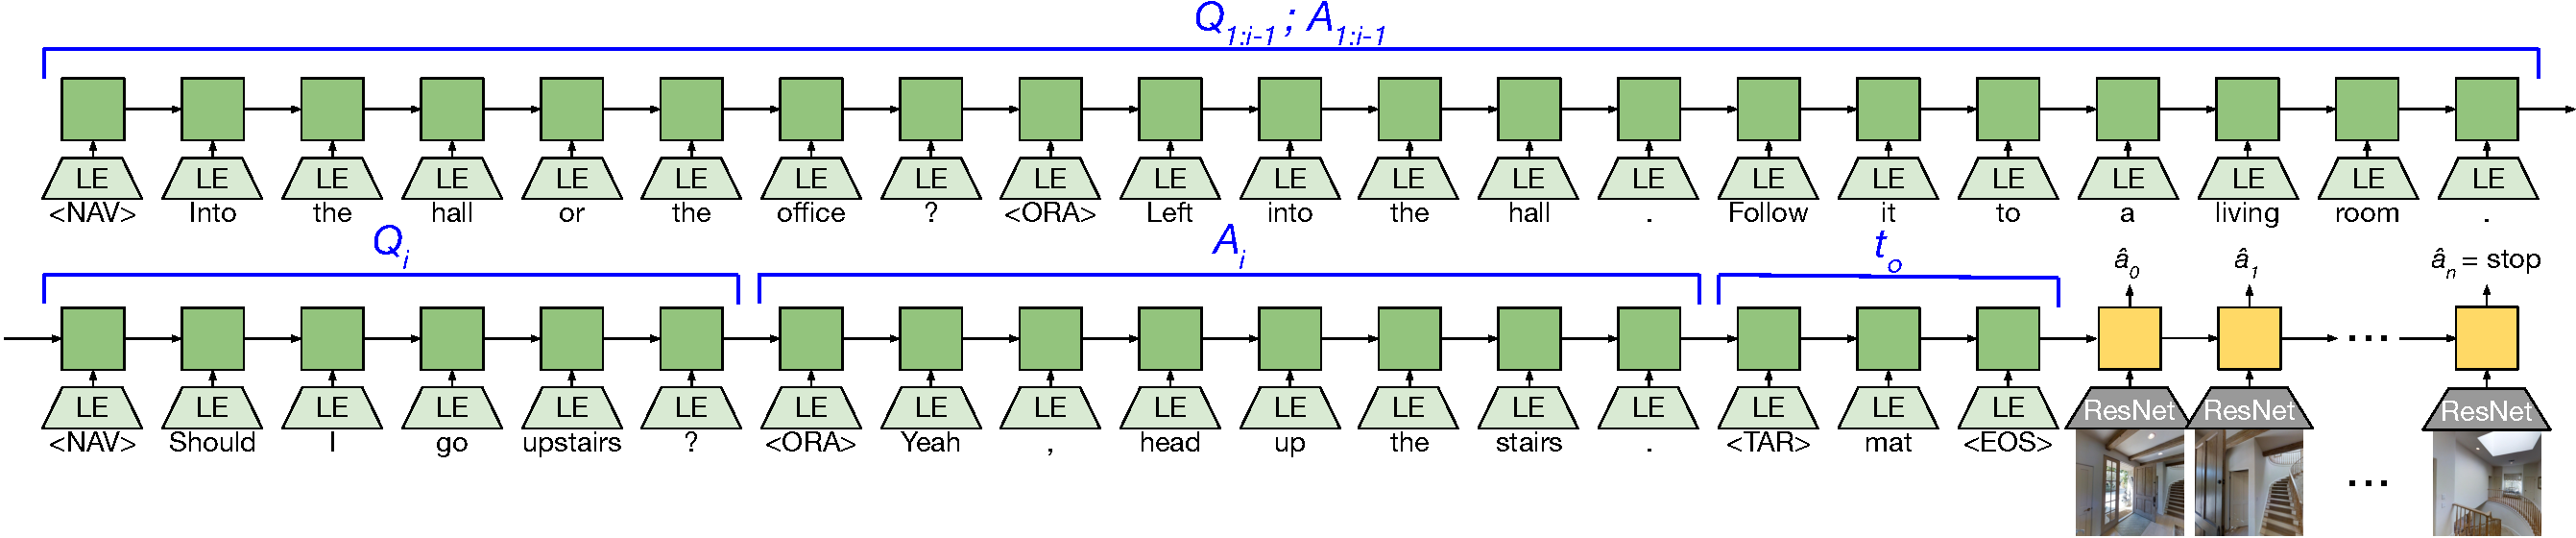
\includegraphics[width=1.\columnwidth]{figures/model.pdf}
\caption{We use a sequence-to-sequence model with an LSTM encoder that takes in learnable token embeddings (LE) of the dialog history.
The encoder conditions an LSTM decoder for predicting navigation actions that takes in fixed ResNet embeddings of visual environment frames.
Here, we demarcate subsequences in the input (e.g., $t_o$) compared during input ablations.
}
\label{fig:model}
\vspace{-3mm}
\end{figure}

We divide these instances into training, validation, and test folds, preserving the R2R folds by house scan.
This division is further done by dialog, such that for every dialog in \dataset{} the \task{} instances created from it all belong to the same fold.
As in R2R, we split the validation fold into \textit{seen} and \textit{unseen} house scans, depending on whether the scan is present in the training set. This results in 4742 training, 382 \textit{seen} validation, 907 \textit{unseen} validation, and 1384 \textit{unseen} test instances.

We provide two forms of supervision for the \task{} task: $N_i$, the navigation steps taken by the \nav{} after question-answer exchange $i$, and $O_i$, the shortest-path steps shown to the \ora{} and used as context to provide answer $A_i$.
In each instance of the task, $i$ indexes the QA exchange in the dialog from which the instance is drawn (with $i=0$ an empty QA followed by initial navigation steps).
Across \task{} instances, the $N_i$ steps range in length from 1 to 40 (average $6.63$), and the $O_i$ steps range in length from 0 to 5 (average $4.35$).
The \nav{} often continues farther than what the \ora{} describes, using their intuition about the house layout to seek the target object.

We evaluate performance on this task by measuring how much progress the agent makes towards $G_j$.
Let $e(P)$ be the end node of path $P$, $b(P)$ the beginning, and $\hat{P}$ the path inferred by the navigation agent.
Then the progress towards the goal is defined as the reduction (in meters) from the distance to the goal region $G_j$ at $b(\hat{P})$ versus at $e(\hat{P})$.
Because $G_j$ is a set of nodes, we take the minimum distance $\min_{p\in G_j}(d_m(p, q))$ as the distance between $q$ and region $G_j$.
Note that this is a topological distance (e.g., we measure the distance around a wall, rather than straight through it).
